\chapter{Implementierung}
Die Implementierung wurde entlang des Entwurfs durchgeführt. Es werden UML Klassen- und Sequenz-Diagramme verwendet, um die Zusammenhänge zu visualisieren.

\section{Überblick}
Im Rahmen der Arbeit sind eine Reihe von Bundles entstanden, die die verschiedenen Funktionalitäten umsetzen. Es lassen sich drei Arten von Bundles unterscheiden:
\begin{enumerate}
\item Die Bundles \textit{tka.binding.core} und \textit{tka.automation.extension} bieten eine Reihe generischer Schnittstellen, die von den Bindings genutzt werden.
\item \textit{tka.binding.twitter}, \textit{tka.binding.dropbox}, \textit{tka.binding.weather} und \textit{tka.binding.gmail} sind Bindings, die jeweils einen konkreten Webservice in das System integrieren. 
\item Das \textit{tka.flashui} Bundle stellt eine Benutzeroberfläche bereit, über die neue Webservice-Things zum System hinzugefügt und durch Regeln automatisiert werden können.
\end{enumerate}


\section{Schnittstellen-Bundles}

\subsection{tka.binding.core}
\label{impl:core}
Das Bundle \textit{tka.binding.core} enthält die zentrale Schnittstelle für den Prozess der Authentifizierung. Sie ist generisch aufgebaut und entspricht den Anforderungen des OAuth Standards (siehe Sektion \ref{subsubsec:oauth}). In Abbildung \ref{fig:connectionservice} ist die Struktur visualisiert.

\begin{figure}[h]
	\centering
	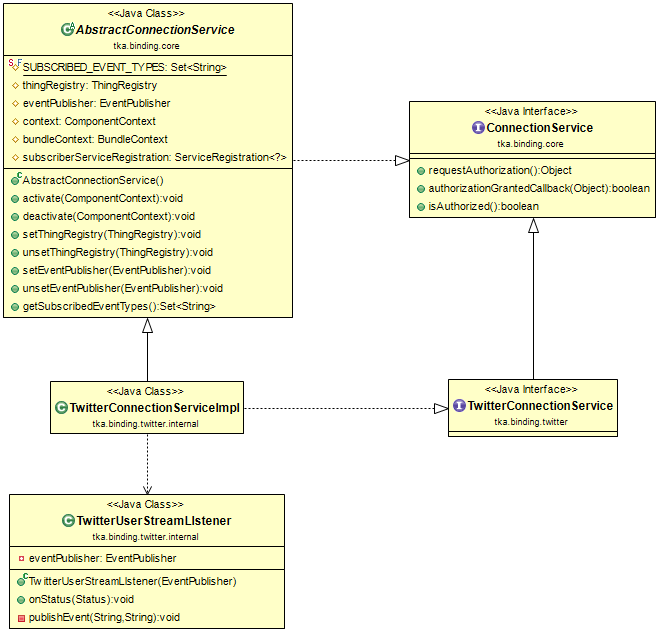
\includegraphics[width=\textwidth]{bilder/ConnectionService}
	\caption{Die Struktur einer Verbindung mit Besipielimplementierung für Twitter}
	\label{fig:connectionservice}
\end{figure}

\subsubsection{ConnectionService}
Die ConnectionService Schnittstelle bietet drei wesentliche Methoden, die bei der Authentifizierung relevant sind. Per \textit{requestAuthorization} teilt der Nutzer mit, dass er wünscht, die Anwendung mit einem seiner Webservice-Accounts (beispielsweise Twitter) zu verknüpfen. Daraufhin bekommt er in der Regel eine URL geliefert, über die er dies umsetzen kann. Die PIN, die er auf diese Weise erhält, teilt er über den \textit{authorizationGrantedCallback} der Anwendung mit. Schließlich lässt sich über \textit{isAuthorized} stets abfragen, ob die Anwendung bereits über die benötigten Zugriffsrechte verfügt. Im Rahmen dieser Arbeit wurde entschieden, sich auf die tatsächliche Unterstützung nur eines Accounts einer Art zu beschränken, obwohl die generische Struktur geeignet ist, um beliebige Mengen von Accounts zu verwalten.

\subsubsection{AbstractConnectionService}
Der AbstractConnectionService bietet eine Reihe von unterstützenden Funktionalitäten, die in der Regel von den Bindings benötigt werden. Hierzu gehört unter anderem die Beziehung des \textit{ThingRegistry}- und \textit{EventPublisher}-Services aus dem System, sowie die eigene Registrierung als \textit{EventSubscriber}. Die ThingRegistry wird benötigt um entsprechende Things im System zu registrieren, nachdem die Autorisierung erfolgreich abgeschlossen ist. Über den EventPublisher publizieren die konkreten Listener (z.B. TwitterUserStreamListener) die Zustandsänderungsevents (mehr dazu in Sektion \ref{sec:bindings_impl}). Als EventSubscriber registriert sich ein ConnectionService um auf Änderungen von Things im System entsprechend reagieren zu können. Beispielsweise, falls ein Thing gelöscht wird, muss auch der zugehörige Listener entfernt werden.\\



Jedes Binding enthält eigene Implementierungen der oben genannten Schnittstellen, die die Besonderheiten des konkreten Webdienstes berücksichtigen. Diese Implementierungen werden außerdem als Services in OSGi registriert, damit über die Benutzeroberfläche die Authentifizierung umgesetzt werden kann.


\subsection{tka.automation.extension}
Das \textit{tka.automation.extension} Bundle registriert im System einige gemeinsamen Services, die von anderen Bundles genutzt werden. Unter anderem wird hier ein neuer Event-Typ registriert: Das \textit{FlashEvent}. Die implementierten Bindings publizieren alle Events dieses Typen, mit unterschiedlichen Topics und Payloads. Dies erlaubt es zu vermeiden, dass jedes Binding seine eigenen Event-Typen deklarieren muss. 


\section{Bindings}
\label{sec:bindings_impl}
Die Bindings sind wie in Sektion \ref{esh:bindings} erläutert aufgebaut. Es wird stets ein neuer Thing-Typ über die \textit{thing-types.xml} im System registriert. Die Anzahl der unterstützten Channels hängt dabei vom jeweiligen Webservice ab.

Jedes Binding integriert einen eigenen Webservice und fügt, sofern notwendig, spezielle Trigger und Actions dem System hinzu. Diese Module erlauben es die Interaktion mit diesen Services über die ESH Rule Engine sinnvoll zu automatisieren.

Alle Bindings haben gemeinsam, dass sie bei den respektiven Webdiensten zunächst registriert werden müssen. Dabei erhalten sie ein Token, mit dem sie sich gegenüber dem Dienst bei Aufrufen identifizieren. Wie komplex dieser Ablauf ist, hängt vom jeweiligen Service ab.

\subsection{tka.binding.twitter}
Das Twitter Binding fügt dem System Things des Typs \glqq twitter\grqq{} hinzu. Es wird derzeit der Channel \glqq status\grqq{} unterstützt. Dies bedeutet, dass es möglich ist über die Rule Engine den aktuellen Status des Nutzers über Regeln zu manipulieren. Die entsprechende Logik ist in dem \textit{TwitterHandler} und der \textit{TwitterAction} hinterlegt. \\

Der \textit{TwitterHandler} ist ein ThingHandler, der konkrete (String-)Commands erhält und dafür verantwortlich ist den Twitter-Status des Nutzers entsprechend zu aktualisieren.  Hierzu liest er sich die Zugriffsdaten aus der Thing-Konfiguration aus und teilt Twitter mit, was geschehen soll.\\

Die \textit{TwitterAction} ist dafür verantwortlich die konkreten Commands zu erzeugen und an den entsprechenden TwitterHandler zu vermitteln. Hierfür erwartet sie eine Reihe von Konfigurationsparametern, die benötigt werden, um eindeutige Befehle zu erstellen. In Tabelle \ref{table:io} ist aufgeführt, welche Eingabeparameter das Modul erwartet.\\

Umgekehrt ist das Binding in der Lage auf viele Zustandsänderungen des Accounts zu reagieren. Die konkrete Logik hierfür ist im \textit{TwitterUserStreamListener} implementiert. So werden unterschiedliche Events publiziert, wenn

\begin{enumerate}
\item sich ein Status, dem der Nutzer auf Twitter folgt, ändert. In diesem Fall wird der neue Status im Payload des Events gespeichert.
\item ein Status sich ändert und Medien (z.B. Bilder) enthält. In diesem Fall wird für jedes Medium ein eigenes Event publiziert, dass die Medien-URL enthält.
\item der Nutzer eine Nachricht erhält. Der Text der Nachricht wird im Payload hinterlegt.
\item viele weiter Ereignisse eintreffen.
\end{enumerate}
 
Falls ein bestimmtes Szenario nicht abgedeckt ist, lässt sich der \textit{TwitterUserStreamListener} entsprechend erweitern.\\



Bei der Interaktion mit Twitter kommt die Twitter4J-Bibliothek\cite{twitter4j} zum Einsatz. Dabei handelt es sich um eine leichtgewichtige Java-Bibliothek, ohne zusätzliche Abhängigkeiten, die die Twitter API 1.1 komplett unterstützt. Sie assistiert zusätzlich bei dem OAuth Prozess.\\



\subsubsection{Überblick über die relevanten Trigger, Conditions und Actions}
\begin{table}[h]
\centering
\begin{tabular}{l|c|r}
	\textbf{Modul Name}  & \textbf{Eingaben} & \textbf{Ausgaben} \\
	GenericEventTrigger  & -        			&  <triggerId>.event   \\ 
    EventCondition		&	event   			&	-\\
    TwitterAction		&	event [itemName, message]	& 	-	\\
    DropboxAction		&	event [itemName, directory, mediaUrl]	& - \\
    EmailAction			&	event [to, subject, message]	& -\\
\end{tabular}
\caption{Eingaben und Ausgaben der relevanten Trigger, Conditions und Actions}
\label{table:io}
\end{table}

In der Tabelle sind die Eingaben und Ausgaben von wichtigen Auslösern, Bedingungen und Aktionen aufgeführt. Zu beachten ist, dass die Eingaben sowohl über den Kontext übergeben, als auch direkt in der Konfiguration der konkreten Instanz fest definiert werden können. Dies erlaubt es sowohl statische als auch generische Regeln zu definieren. Falls Parameter fehlen sollten, wird die konkret betroffene Aktion nicht ausgeführt, der gesamte Ausführungsprozess wird nicht unterbrochen.

\subsection{tka.binding.dropbox}
Das Bundle \textit{tka.binding.dropbox} ist analog zu \textit{tka.binding.twitter} aufgebaut. Es wird der neue Thing-Typ \glqq dropbox\grqq{} mit dem Channel \glqq folder\grqq{} im System registriert. Über diesen Channel gibt es die Möglichkeit neue Dateien in die Dropbox hochzuladen. \\

Der \textit{DropboxChangesTracker} übernimmt die Rolle des \textit{TwitterUserStreamListeners}. Er überprüft alle 5 Sekunden den Inhalt der Dropbox und publiziert Events für sämtliche Änderungen.\\

Über die \textit{DropboxAction} lassen sich neue Dateien automatisch in die Dropbox hochladen. Beispielsweise kann eine Regel erstellt werden, die mit Hilfe eines GenericEventTriggers auf vom Twitter-Binding publizierte (Medien-)Events reagiert und daraufhin über die Medien-URL die Datei an einem spezifizierten Ort speichert.\\

Bei der Interaktion mit dem Webservice kommt die vom Hersteller angebotene Dropbox SDK zum Einsatz. Dabei handelt es sich um eine Java-Bibliothek, die den Entwickler bei der OAuth-Authentifizierung und der gesamten Interaktion mit Dropbox (Hochladen und Löschen von Dateien, etc.) unterstützt. 

Diese externen Bibliotheken (Dropbox SDK, Twitter4J) wurden mithilfe des bnd-Tools\cite{bnd} zu OSGi-Bundles umgewandelt. Dabei stellte sich heraus, dass die Dropbox SDK Abhängigkeiten auf eine Reihe von Android Bibliotheken besitzt. Nach weiterer Recherche ließen sich diese Abhängigkeiten mithilfe des bnd-Tools auf optional umstellen, wonach die SDK problemlos in der OSGi Umgebung eingesetzt werden konnte. 




\subsection{tka.binding.weather}
Das \textit{tka.binding.weather} Binding weist sowohl Gemeinsamkeiten, als auch Unterschiede zu den bisher vorgestellten Bundles auf. Es handelt sich bei dem Wetterdienst um einen Webservice, der einer regulären intelligenten Wetterstation stark ähnelt. Dadurch ließen sich mehr Funktionalitäten von ESH wiederverwenden, als bei den anderen Diensten.

Gleichzeitig unterscheidet es sich von den bisher vorgestellten dadurch, dass es sich bei dem Webservice um einen öffentlichen Dienst handelt. Das bedeutet, dass ein komplexer Autorisierungsprozess (beispielsweise über OAuth) an dieser Stelle nicht benötigt wird. Dies führt dazu, dass keine eigene Implementierung der in Sektion \ref{impl:core} vorgestellten Schnittstellen notwendig ist. 

Das Binding registriert den neuen Thing-Typen \glqq weather\grqq{} mit den Channels \textit{temperature}, \textit{humidity} und \textit{rain}. 

Da die Zustandsaktualisierung in diesem Fall vergleichsweise simpel verläuft, wurde sie nicht in eine dedizierte Klasse ausgelagert. Stattdessen wurde der ThingHandler um die entsprechende Funktionalität erweitert. Da sich das Wetter von Region zu Region mit sehr unterschiedlicher Geschwindigkeit ändern kann, lässt sich die Aktualisierungsperiode über die Benutzeroberfläche beliebig konfigurieren.


\subsection{tka.binding.gmail}
Das Bundle \textit{tka.binding.gmail} erlaubt es dem Nutzer Emails zu versenden. Es ist analog zu den bisherigen Bindings aufgebaut. Der Thing-Typ \glqq gmail\grqq{} wird im System registriert und über einen entsprechenden ThingHandler gesteuert. 

Das Binding registriert den Action Typen \textit{EmailAction}, über den der Nutzer angeben kann, an wen eine Email mit den gewählten Informationen gesendet werden soll. Die Email wird von einer anwendungsinternen Google Mail\cite{gmail} Adresse \textit{noreply.flash.ma@gmail.com} über einen öffentlichen SMTP Server versandt.



\section{Benutzeroberfläche}
Die Benutzeroberfläche ist komplett im Bundle \textit{tka.flashui} realisiert. Das Bundle ist von den Bindings los gekoppelt - es nutzt einige der von ihnen bereitgestellten Services um eine rudimentäre, aber dennoch voll funktionsfähige GUI bereitzustellen. Es ist jederzeit möglich diese Benutzeroberfläche auszutauschen oder weitere Schnittstellen parallel im System zu registrieren.


\subsection{tka.flashui}
Aus technischer Sicht wurde die GUI größtenteils über REST-Schnittstellen, Javascript und AJAX realisiert.

\subsubsection{Backend}
Seitens des Backends wird vom OSGi Container ein HTTP-Service bezogen, sowie die von den Bundles bereitgestellten konkreten ConnectionServices. Daraufhin wird in Form von Servlets eine Reihe von Schnittstellen definiert, über die verschiedene Informationen aus dem Frontend per AJAX abgefragt werden können. Auf diese Weise werden Informationen über die aktuell im System verwalteten Rules und Things bereitgestellt. Für jedes Binding gibt es ein eigenes Servlet, das die Interaktion damit (hauptsächlich für die Authentifizierung) ermöglicht. 

\subsubsection{Frontend}
Bei dem Frontend handelt es sich um eine Single-Page-Webanwendung. Es gibt eine HTML-Datei, die ein leeres Grundgerüst für die Seite bietet und eine Reihe von Javascript Dateien, die beim Öffnen der Seite geladen werden. Die verschiedenen logischen Aspekte der  Anwendung werden in separaten JS-Dateien realisiert. Für jedes Binding gibt es ebenfalls eine einzelne JS-Datei, in der die Logik der Zusammenarbeit mit dem konkreten Binding realisiert ist. \\

Das Erweitern der GUI um neue Bindings lässt sich damit auf eine einfache Art und Weise realisieren, ohne existierenden Code ändern zu müssen. Seitens des Backends muss für ein neues Binding eine neue REST-Schnittstelle in Form eines Servlets definiert werden. Das Frontend bedarf	einer lediglich einer weiteren JS-Datei.		\\


\subsubsection{Funktionalität und visuelle Darstellung}
Die Benutzeroberfläche bietet die Möglichkeit die implementierten Funktionalitäten zur Laufzeit zu konfigurieren. Sie ist in Abbildung \ref{fig:gui_all} dargestellt. 

\begin{figure}[h]
	\centering
	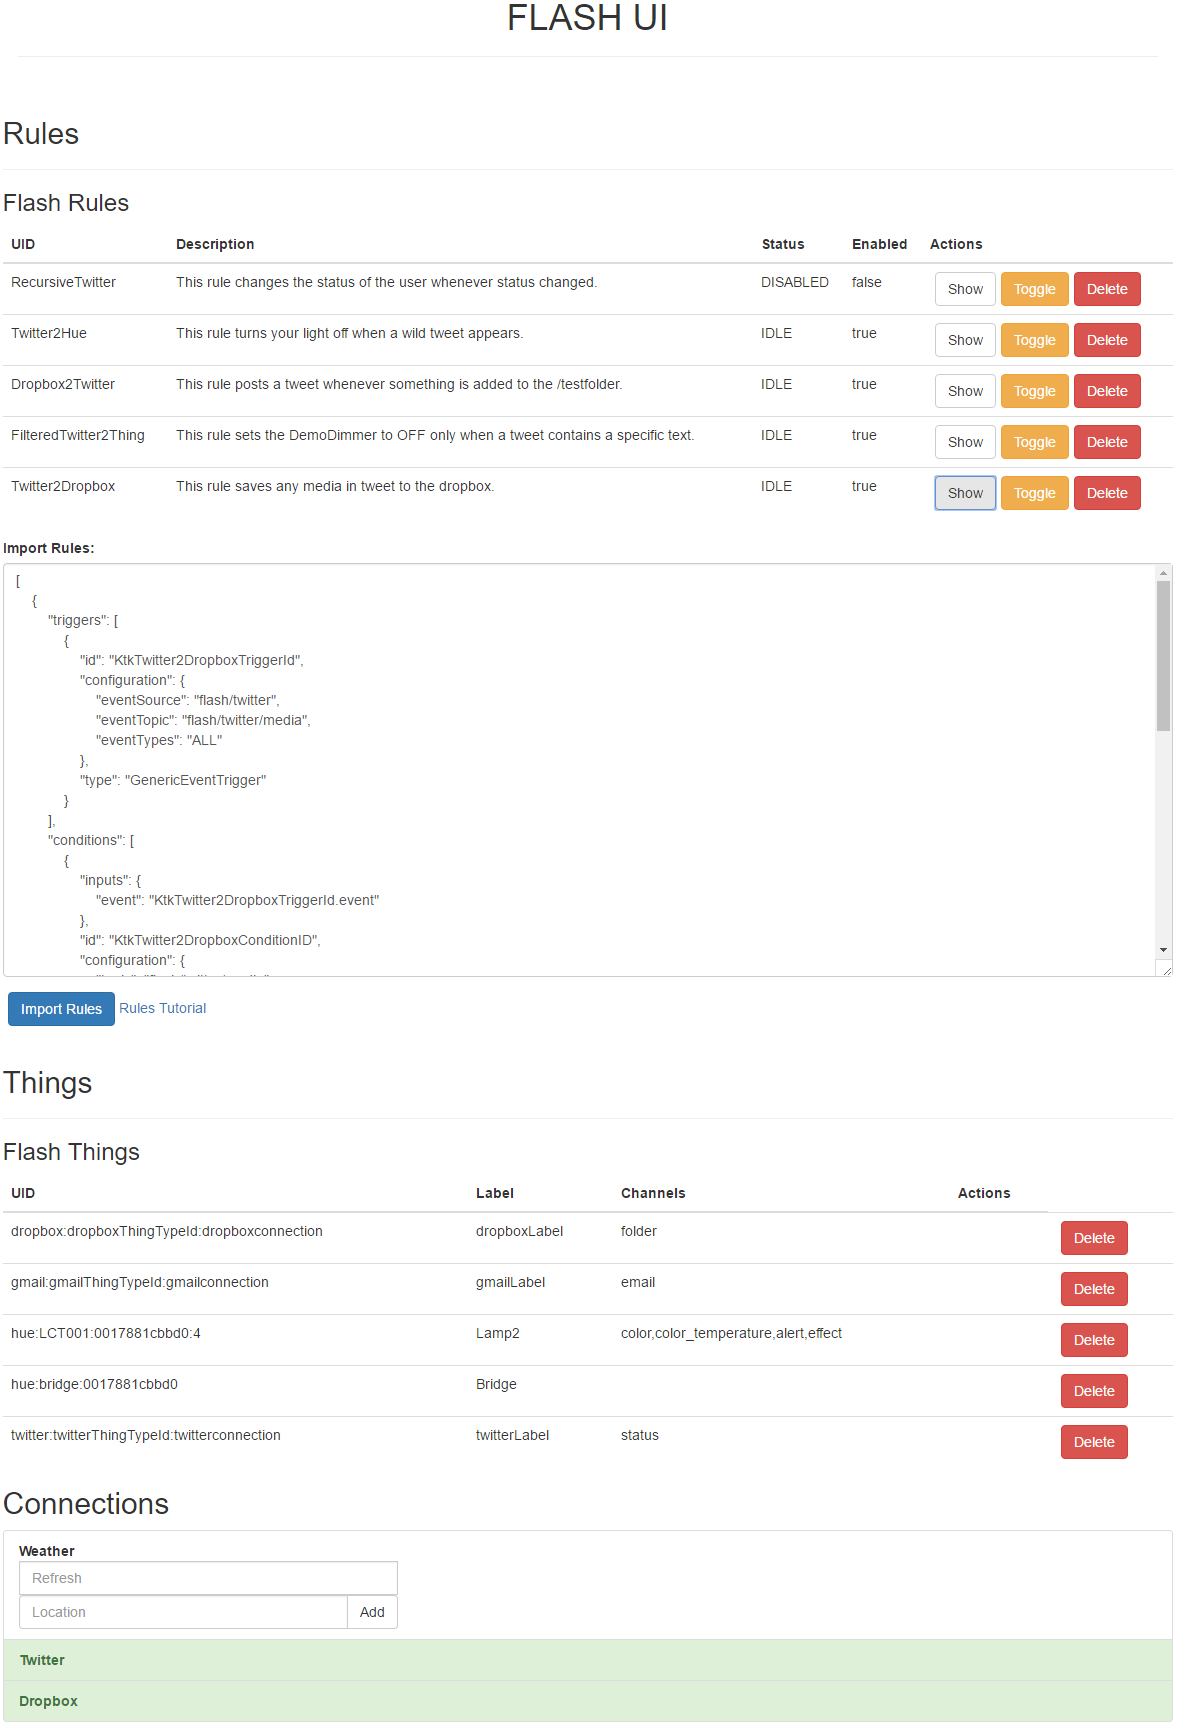
\includegraphics[width=\textwidth]{bilder/gui_all4}
	\caption{Die Benutzeroberlärche}
	\label{fig:gui_all}
\end{figure}

Es ist leicht zu sehen, dass die Oberfläche grob in drei Abschnitte unterteilt werden kann. Im Abschnitt \textit{Rules} gibt eine Tabelle mit den aktuell existierenden Regeln zu sehen, sowie der Möglichkeit, diese Regeln zu manipulieren. Neue Regeln können im JSON-Format konfiguriert und über \textit{Import Rules} an das Backend übermittelt werden. Sie werden daraufhin mithilfe von GSON\cite{gson} zu Rules umgewandelt und dem System hinzugefügt. Auf diese Weise importierte Regeln überschreiben existierende Regeln mit der gleichen Id.

Im Abschnitt \textit{Things} sind die aktuell im System vorhandenen Things mit den von ihnen unterstützten Channels zu sehen. 

Im letzten Teil der Benutzeroberfläche ist eine Liste mit den unterstützten Webservices bereitgestellt. Für jeden Webdienst gibt es hier die Möglichkeit die Zugriffsrechte an die Anwendung zu vermitteln.

Beim Stylen der Oberfläche kam Bootstrap\cite{bootstrap} zum Einsatz.


\section{Deployment auf dem Raspberry Pi}
\label{impl:deployment}
Das Deployment fand auf einem Raspberry Pi 3 Model B statt. Auf dem Gerät lief das Betriebssystem \textit{Raspbian} mit installiertem Java 8.

Als Grundlage für die Distribution wurde das \textit{Eclipse SmartHome Packaging Sample}\cite{eshsample} verwendet. Es erlaubt es mithilfe von Maven\cite{maven} eine leichtgewichtigen OSGi Container mitsamt einigen der zusätzlich benötigten Services zu bauen. Diese Distribution wurde entsprechend angepasst: 
\begin{enumerate}
\item Weitere notwendige Service-Bundles wurden hinzugefügt. Vor allem bei dem Einbinden von den externen Bibliotheken (Dropbox SDK und Twitter4J) mussten an dieser Stelle zusätzliche Konfigurationen vorgenommen werden.
\item Die eigenen Bundles wurden mithilfe von Maven zu OSGi-Jar-Dateien umgewandelt und zum Deployment hinzugefügt.
\end{enumerate}

Schließlich wurde die Distribution auf dem Raspberry Pi gestartet und und einem umfangreichen Test unterzogen. Die Ergebnisse dieses Tests werden in Kapitel \ref{chap:eval} vorgestellt.


\section{Fazit}
Die Implementierung wurde entlang des in Kapitel \ref{chap:entwurf} definierten Entwurfs umgesetzt. Sie ist generisch aufgebaut und lässt sich leicht um neue Funktionalitäten erweitern.
